\section{Performance evaluation}

\subsection{Test environment}
\subsubsection{Pianosa}
\subsubsection{''Physics cluster''}

\subsection{Performance measurement approach}
\label{test-env}
There are two different approaches to measure performance: profiling and benchmarking.

Profiling is used to measure the performance of a given application by adding time measuring and logging code. After the execution has been completed, one can retrace and check how much time had been spent in which function call. This is useful for application developers to find potential bottlenecks and inefficient implemented functions.

Benchmarking addresses mainly the levels underneath the application level, for instance the performance
of the MPI-implementation, the performance of the network and devices. Most interesting results are latencies and bandwidths and their course for various packet or messages sizes. Benchmarking is done by performing numerous iterations of computation and/or communication and measuring the elapsed time.

We used the latter technique to measure the performance of the two message-passing environments, and a combination of both benchmarking and profiling techniques to measure the performance of the different sorting algorithms.

\subsection{MPI cost model}
In a simplified view, the cost of sending a message between two tasks located on different processors can be represented by two parameters: the message startup time $T_{setup}$, which is the time required to initiate the communication, and the transmission time $T_{trasm}$ per word, which is determined by the physical bandwidth of the communication channel linking the source and destination processors. The time required to send a message of size L words is then
\[
T_{send} = T_{setup} + L * T_{trasm}
\]
While accurate for many algorithms and on many architectures, this model can break down if a computer's interconnection network has particular properties, especially if an application generates many messages.
\\ \\
/* \dots \textit{TODO} \dots */
\\ \\
In order to benchmark the performance of the two environments, we decided to use the \textit{Perftest} benchmark suite.

The perftest-package is provided along with the MPI-implementation MPICH, although it can be used in combination with any MPI-implementation. The package contains a few tools to measure the performance of a message passing environment. The two major programs are \textit{mpptest} for measuring point-to-point communication and \textit{goptest} for measuring collective communication. In addition to the classic ping-pong test, mpptest can measure performance with many participating processes (exposing contention and scalability problems) and can adaptively choose the message sizes in order to isolate sudden changes in performance. 

The following test were performed:
\begin{itemize}
	\item Round-trip times between 2 nodes using blocking methods
	\item Blocking bisection times involving from 4 to $n$ nodes
	\item Broadcast times involving from 2 to $n$ nodes
\end{itemize}
In the bisection test the complete system is logically divided into two subsystems and the aggregated bandwidth and latency between the two subsystems is measured. An example of this is splitting the system in two vertically and letting each node in the left half communicate with a node in the right part on a one-to-one basis.


\subsubsection*{Pianosa}
\label{test-env-pianosa}
Below are the results obtained on Pianosa:
%\begin{figure}[h!]
%	\centering
%  	\subfloat[Messages of length from 0 to 32 bytes (stride 4 bytes).]{\label{tsend_32}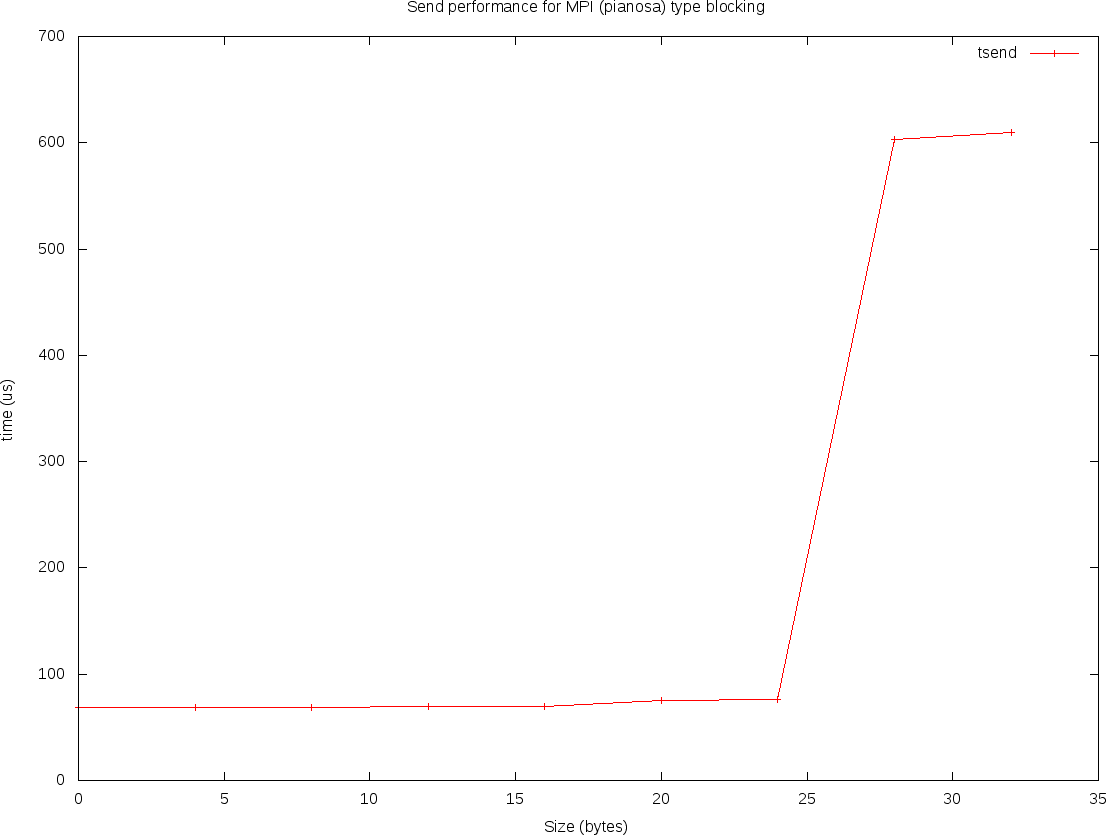
\includegraphics[width=0.5\textwidth]{../tests/mpi_comm_perf/pianosa/tsend_4.png}}  
%	\hspace*{20pt}
%  	\subfloat[Messages of length from 0 to 1024 bytes (stride 32 bytes).]{\label{tsend_32}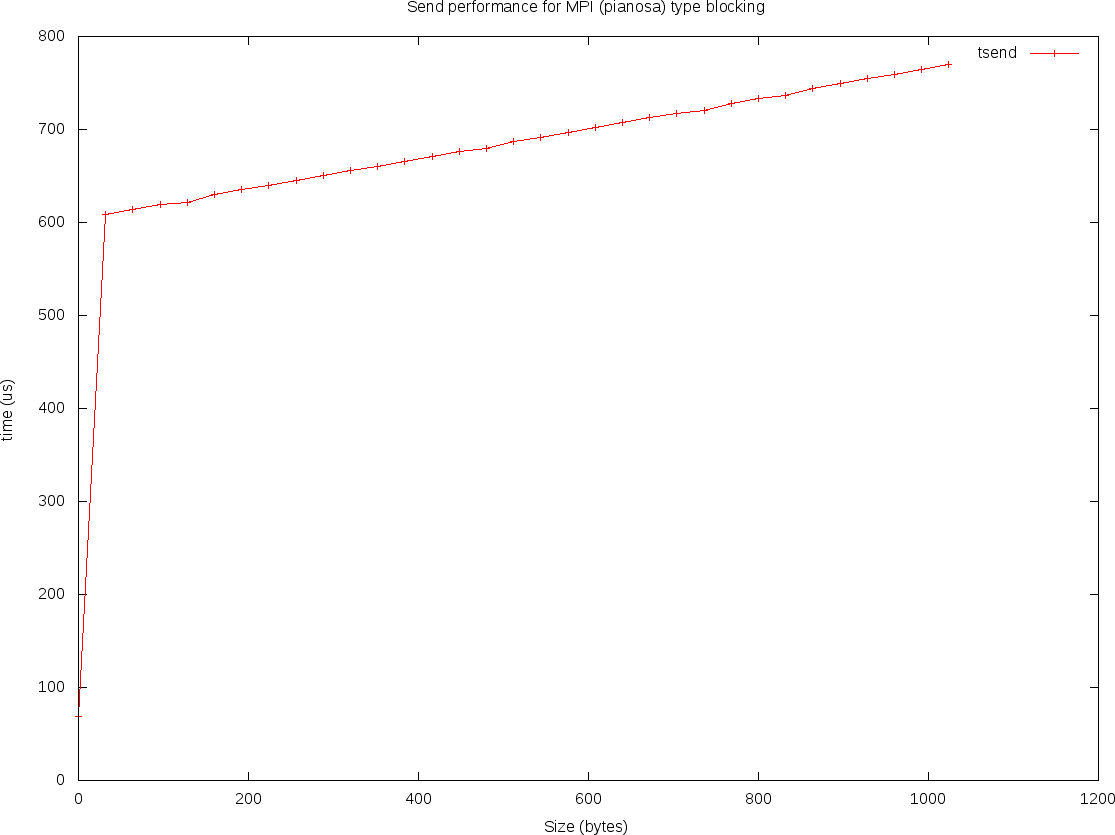
\includegraphics[width=0.5\textwidth]{../tests/mpi_comm_perf/pianosa/tsend_32.png}}  
%	\caption{Performance of blocking send between two processes.}
%\end{figure}
%
%
%\begin{figure}[h!]
%	\centering
%  	\subfloat[Messages of length from 0 to 32768 bytes (stride $2^i$).]{\label{tsend_logscale}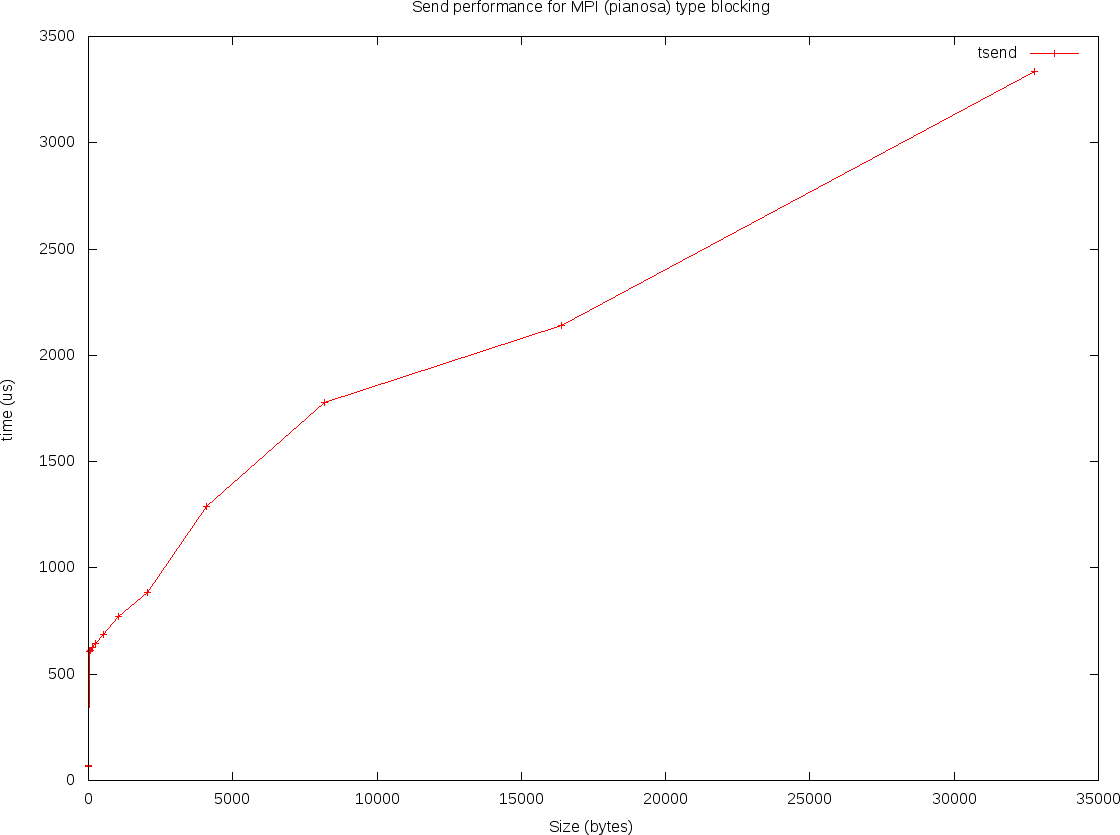
\includegraphics[width=0.5\textwidth]{../tests/mpi_comm_perf/pianosa/tsend_logscale.png}}  
%	\hspace*{20pt}
%  	\subfloat[Bisection test with 4, 8 and 16 processors.]{\label{bisect_logscale}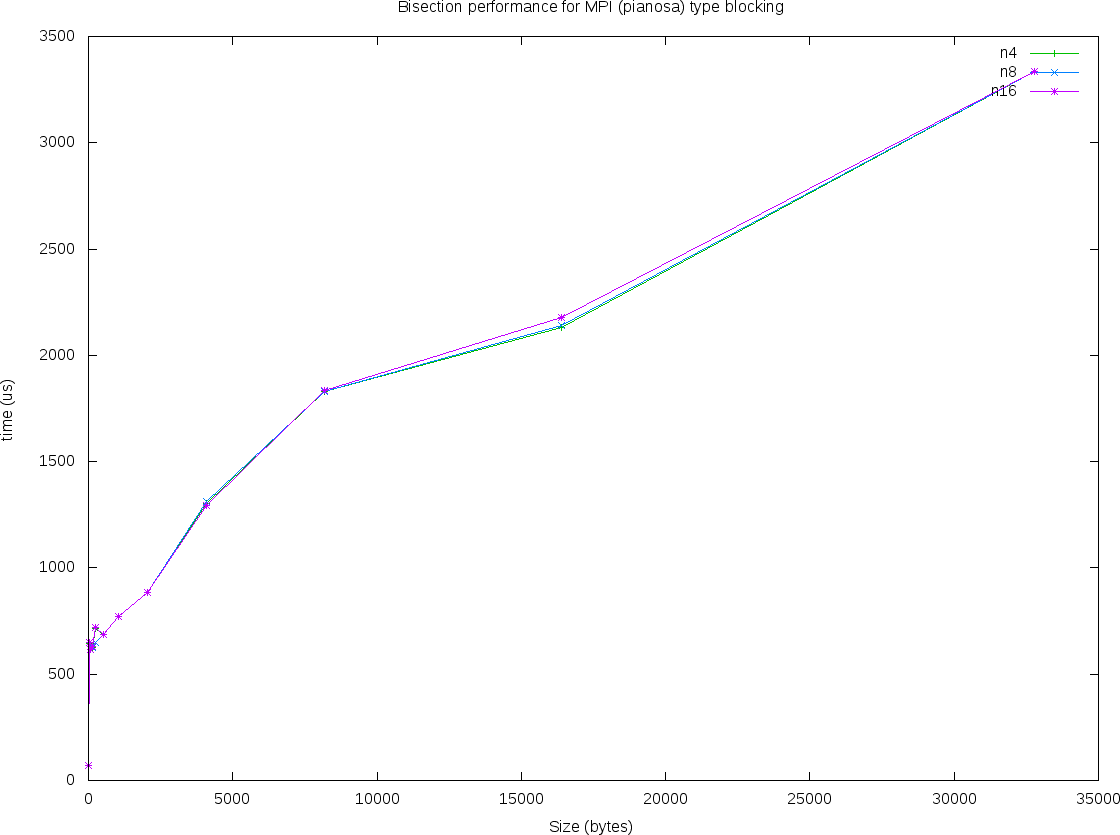
\includegraphics[width=0.5\textwidth]{../tests/mpi_comm_perf/pianosa/bisect_logscale.png}}  
%	\caption{Performance of blocking send and bisection test.}
%\end{figure}
%
%\begin{figure}[h!]
%	\centering {\label{bcast}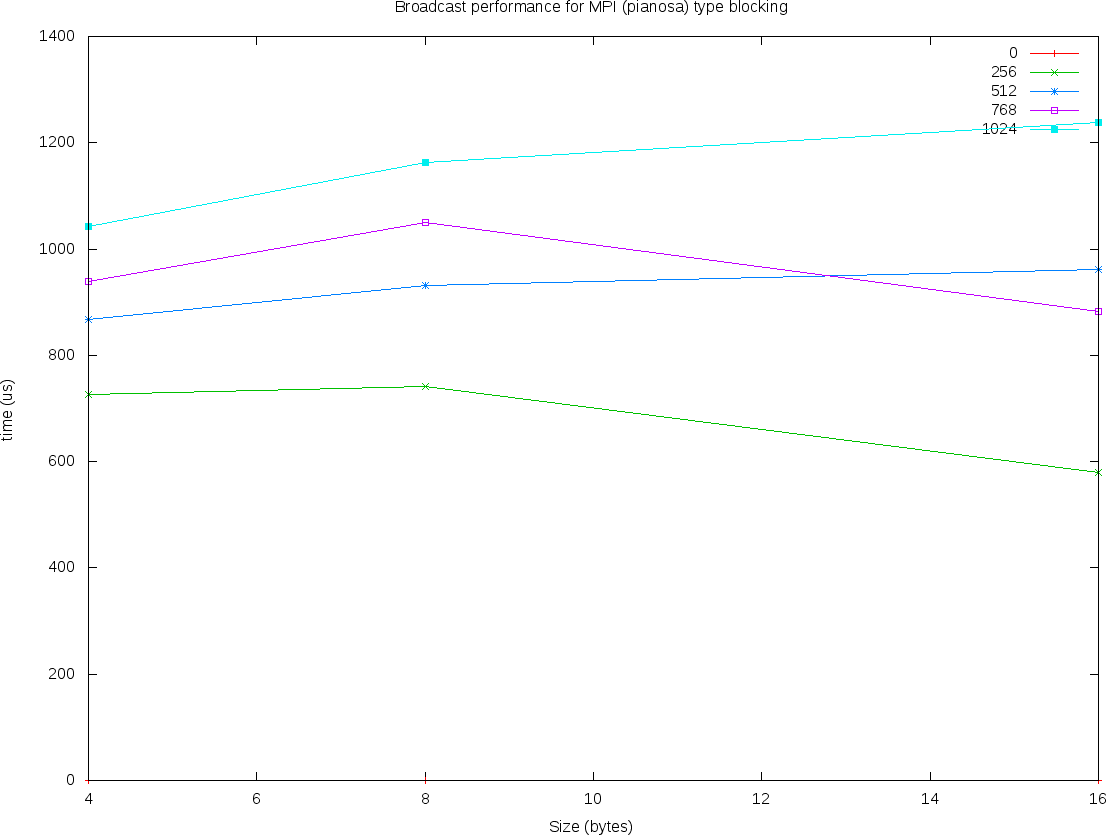
\includegraphics[width=0.5\textwidth]{../tests/mpi_comm_perf/pianosa/bcast.png}}  
%	\caption{Performance of broadcast with 4, 8 and 16 processors.}
%\end{figure}


\begin{figure}[p]
	\centering
  	\subfloat[Messages of length from 0 to 32 bytes (stride 4 bytes).]{\label{tsend_32}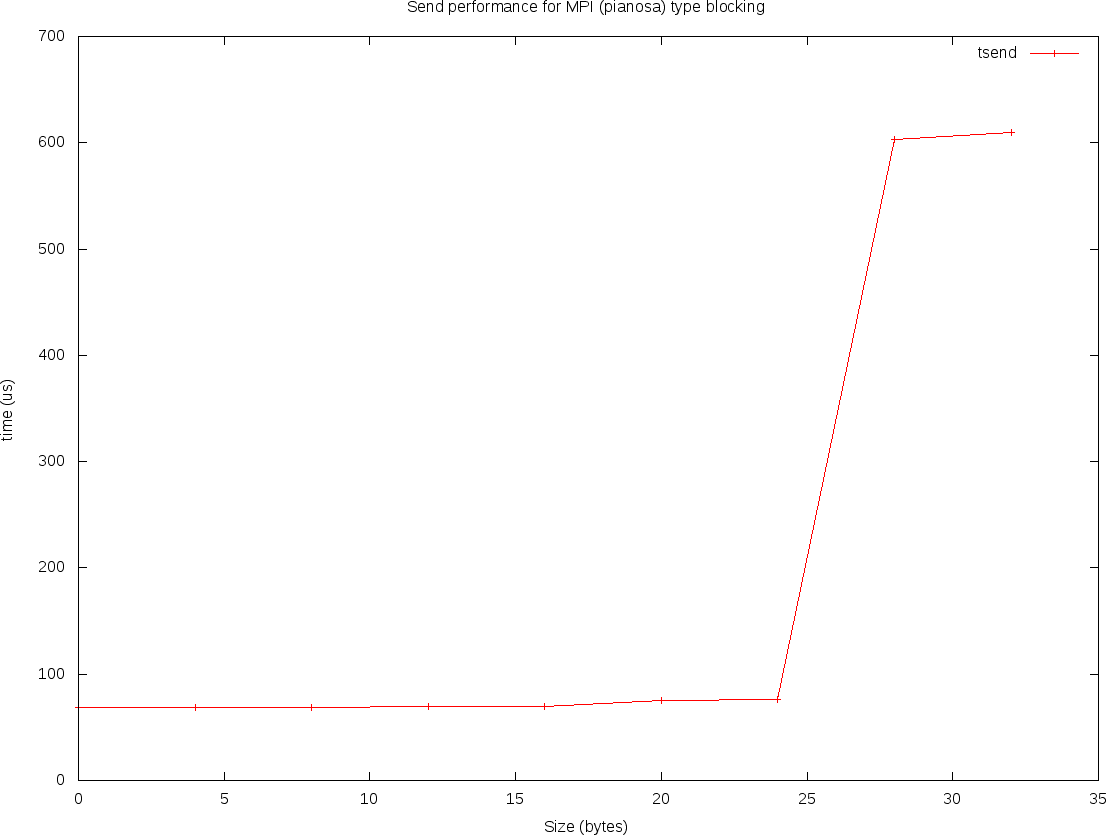
\includegraphics[width=0.4\textwidth]{../tests/mpi_comm_perf/pianosa/tsend_4.png}}  
	\hspace*{20pt}
  	\subfloat[Messages of length from 0 to 1024 bytes (stride 32 bytes).]{\label{tsend_32}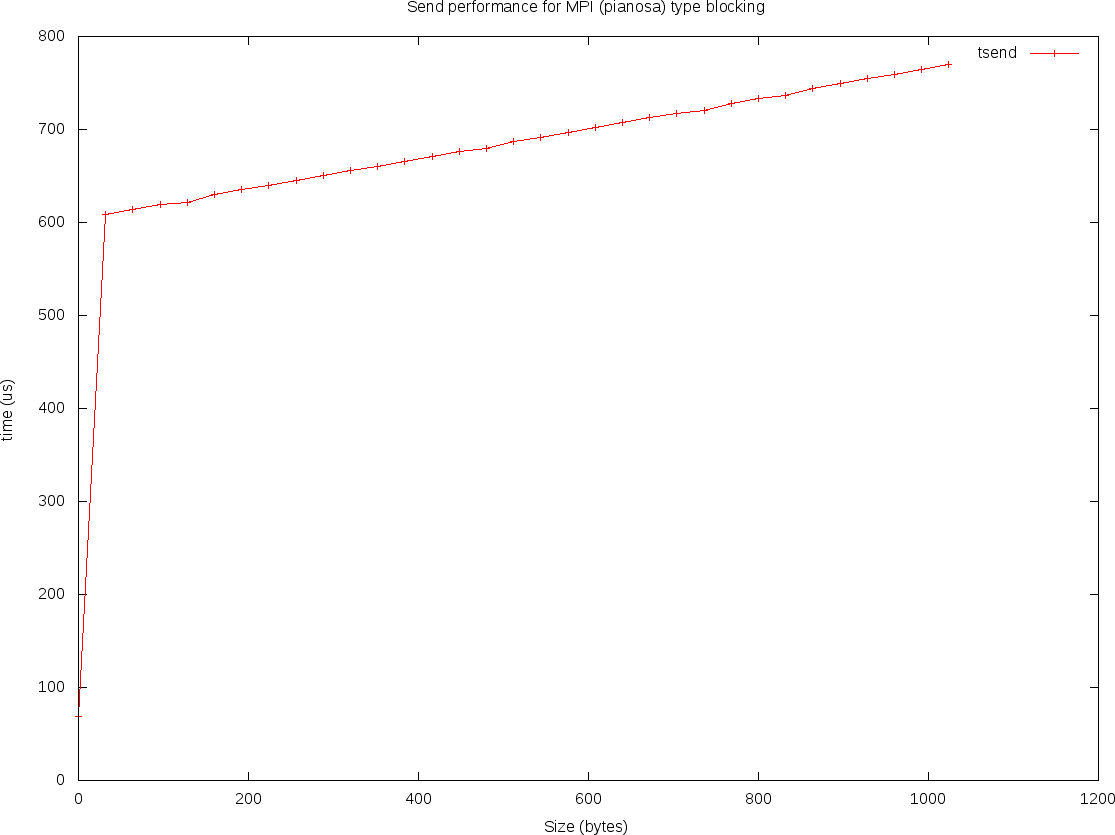
\includegraphics[width=0.4\textwidth]{../tests/mpi_comm_perf/pianosa/tsend_32.png}}  
	\caption{Performance of blocking send between two processes.}
	
	\centering
  	\subfloat[Messages of length from 0 to 32768 bytes (stride $2^i$).]{\label{tsend_logscale}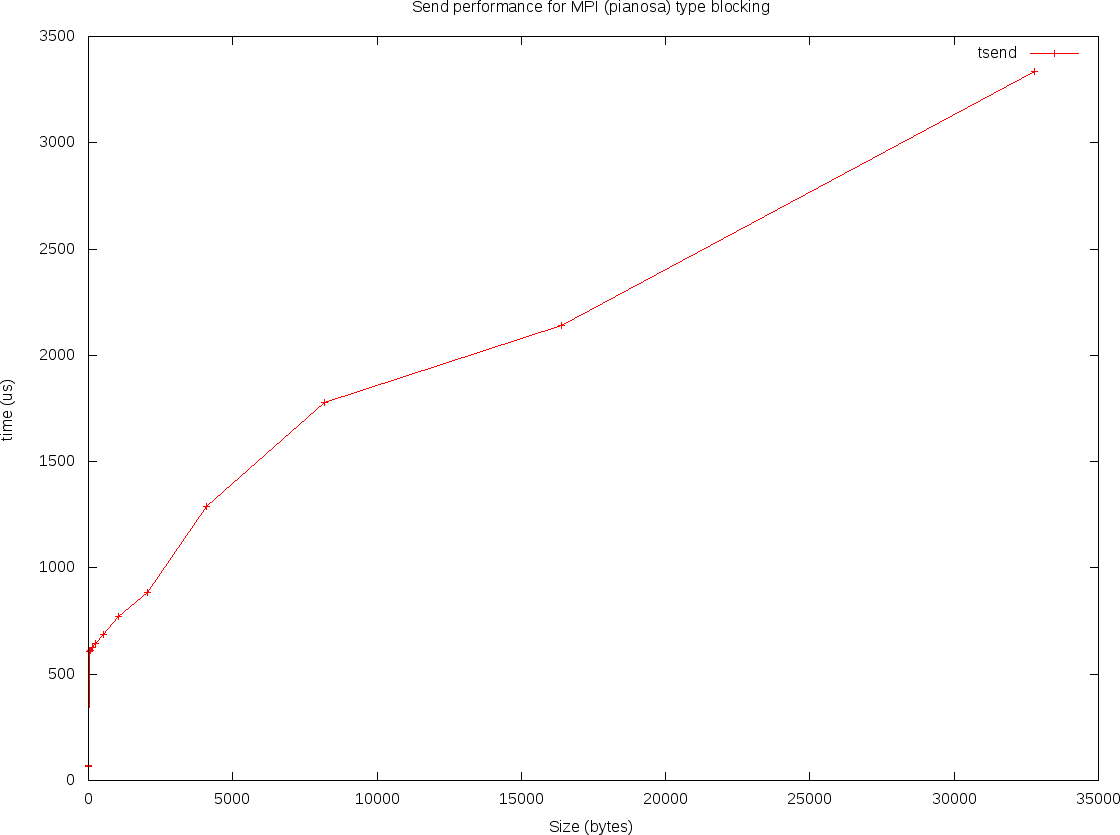
\includegraphics[width=0.4\textwidth]{../tests/mpi_comm_perf/pianosa/tsend_logscale.png}}  
	\hspace*{20pt}
  	\subfloat[Bisection test with 4, 8 and 16 processors.]{\label{bisect_logscale}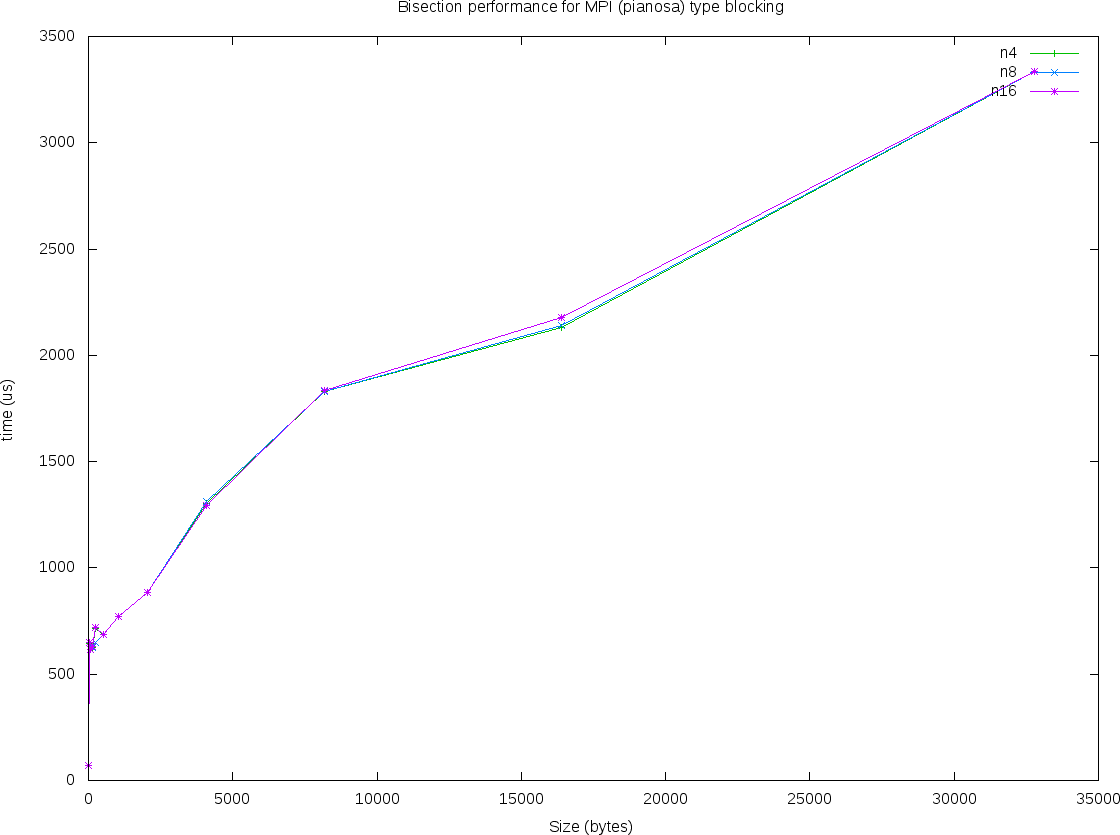
\includegraphics[width=0.4\textwidth]{../tests/mpi_comm_perf/pianosa/bisect_logscale.png}}  
	\caption{Performance of blocking send and bisection test.}
	
	\centering {\label{bcast}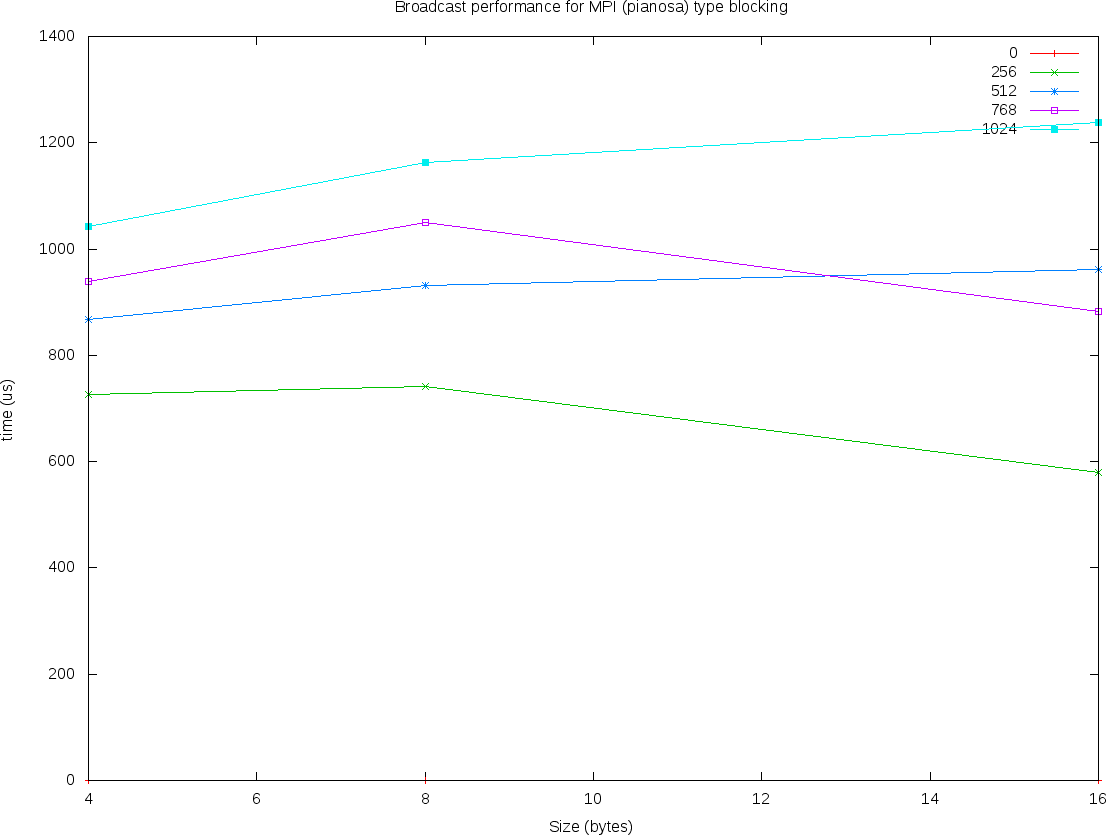
\includegraphics[width=0.4\textwidth]{../tests/mpi_comm_perf/pianosa/bcast.png}}  
	\caption{Performance of broadcast with 4, 8 and 16 processors.}
\end{figure}